% Creating a simple Title Page in Beamer
\documentclass{beamer}
\usepackage{algorithm}
\usepackage[noend]{algpseudocode}
\usepackage[utf8]{inputenc}
\usepackage[bulgarian]{babel}
\usepackage{amsmath,amssymb,amsthm}
\usepackage{graphicx}
\usepackage{subfigure}
\usepackage{pdfpages}
\usepackage{multirow}
\usepackage{adjustbox}
\usepackage{textgreek}
\usepackage{caption}

% Theme choice:
\usetheme{Madrid}
% Title page details: 
\title[]{Имплементация на МКЕ за решаване на уравненията на Навие-Стокс за графични процесори}
\subtitle{\textbf{Защита на дипломна работа}\\
\small{МП \glqq Изчислителна математика и математическо моделиранe\grqq}}
\author[]{Дипломант:~Васил~Пашов,~ФН~25938\\ \and
Научен~ръководител:~гл.~ас.~д-р~Тихомир Иванов}
\date{30 ноември 2021г.}
\newcommand{\norm}[1]{\left\lVert#1\right\rVert}
\newcommand{\dotprod}[2]{\left(#1, #2\right)}
\newcommand{\divg}[1]{\nabla\cdot#1}
\newcommand{\grad}[1]{\nabla#1}
\newcommand{\lapl}[1]{\Delta#1}
\newcommand{\vecf}[1]{\textbf{#1}}
\begin{document}
% Title page frame
\begin{frame}
    \titlepage
\end{frame}

%\begin{frame}{Съдържание}
%    \tableofcontents[hidesubsections]
%\end{frame}
%\AtBeginSubsection[]
%{
%\begin{frame}{\secname}
%	\small
	%\tableofcontents[currentsubsection]
%    \tableofcontents[subsectionstyle=show/shaded/hide]
%\end{frame}
%}
% Presentation structure
\section{Въведение}
\subsection{Уравнения на Навие-Стокс}
\begin{frame}{Уравнения на Навие-Стокс}
\begin{align*}
  % Conservation of momentum
  \frac{\partial \vecf{u}(\vecf{x}, t)}{\partial t} + (\vecf{u}(\vecf{x}, t)\cdot\nabla)\vecf{u}(\vecf{x}, t) + \nabla p(\vecf{x}, t) - \nu\Delta\vecf{u}(\vecf{x}, t) &= \vecf{f}(\vecf{x}, t)\\
  % Continuity
  \nabla \cdot \vecf{u}(\vecf{x}, t) &= 0
\end{align*}
\begin{itemize}
  \item $\vecf{u} \in \mathbb{R}^n$ е скоростта
  \item $p \in \mathbb{R}$ е налягането
  \item $\nu$ е вискозитет
  \item $\vecf{f}$ е съвкупност от обемни сили, напр. гравитация
\end{itemize}
\end{frame}
\subsection{Моделна задача (2D DFG Benchmark)}
\begin{frame}{Моделна задача (2D DFG Benchmark)}
\begin{figure}[H]
  \centering
  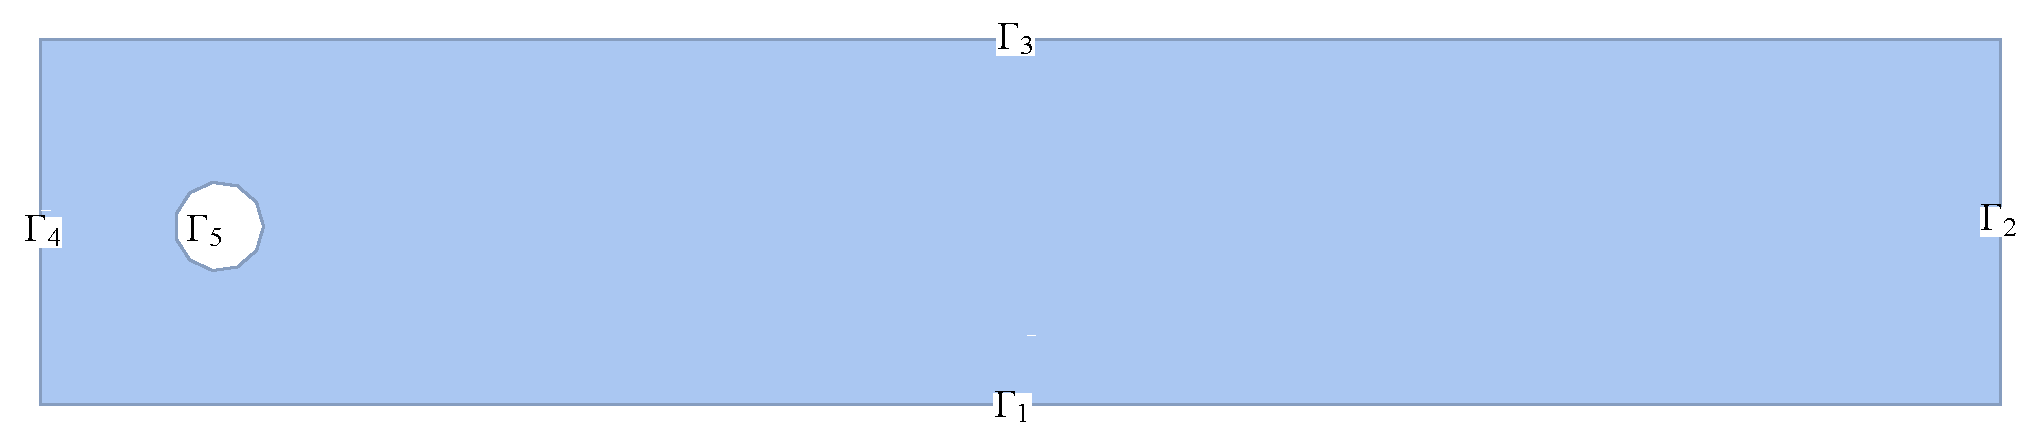
\includegraphics[width=\textwidth]{../Figures/02_model_problem/2D_DFG_Benchmark.pdf}
  % \caption{Геометрия на моделната задача 2D DFG Benchmark}
\end{figure}
Гранични условия:
\begin{align*}
  &\vecf{u} = 0, &&\left(\vecf{x}, t\right) \in \left(\Gamma_1 \cup \Gamma_3 \cup \Gamma_5\right) \times J \\
  &\vecf{u} = \left(\frac{1.2y\left(0.41 - y\right)}{0.41^2}, 0\right), &&\left(\vecf{x}, t\right) \in \Gamma_4 \times J \\
  &\nu\frac{\partial\vecf{u}}{\partial\vecf{n}} - p\vecf{n} = 0, &&\left(\vecf{x}, t\right) \in \Gamma_2 \times J
\end{align*}
Дефинираме $\Gamma_D = \Gamma_1 \cup \Gamma_3 \cup \Gamma_4 \cup \Gamma_5$
\end{frame}

\section{Метод на крайните елементи}





\iffalse
    \subsection{Директен подход}
    \begin{frame}{Директен подход -- слаба формулировка}
    Тестови пространства:
    \begin{itemize}
    		\item $\mathbf{v} \in V : \left\{\mathbf{v} \in H^1 : \mathbf{v}(\mathbf{x}, t)|_{\Gamma_D} = 0 \right\}$
    		\item $p \in L^2(\Omega)$
    \end{itemize}
    Търсим:
    \begin{itemize}
    		\item $\mathbf{u} \in U : \left\{\mathbf{v} \in H^1 : \mathbf{v}(\mathbf{x}, t)|_{\Gamma_1 \cup \Gamma_3 \cup \Gamma_5} = 0\right\}$
    		\item $p \in L^2(\Omega)$
    \end{itemize}
    Такива че:
\begin{align*}
  &\left(\frac{\partial\mathbf{u}}{\partial t}, \mathbf{v}\right)
  + (\mathbf{u}\cdot\nabla\mathbf{u}, \mathbf{v}) + \nu(\nabla\mathbf{u} : \nabla\mathbf{v}) =
  (p, \nabla \cdot \mathbf{v}), &&\mathbf{v} \in V \\
  &(\nabla\cdot\mathbf{u}, q) = 0, &&q \in L^2 \\
  &\mathbf{u} = \mathbf{u_{\Gamma_4}}, &&\left(\mathbf{x}, t\right) \in \Gamma_4 \times J  
\end{align*}
    \end{frame}
    \begin{frame}{Директен подход -- метод на крайните елементи}
    		Дефинираме крайномерните пространства $U_h$ и $L_h$
		\begin{itemize}
			\item $U_h = span\left\{
								\begin{bmatrix} \phi_1 \\ 0\end{bmatrix}
								, \dots ,
								\begin{bmatrix} \phi_{N_v} \\ 0\end{bmatrix} ,
								\begin{bmatrix} 0 \\ \phi_1\end{bmatrix}
								, \dots ,
								\begin{bmatrix} 0 \\ \phi_{N_v}\end{bmatrix}
						\right\}$
  			\item $L_h = span\left\{\chi_i\right\}^{N_p}_{i = 1}$
		\end{itemize}
    		Търсим приближени решения за скоростта и налягането:
    		\begin{itemize}
    			\item $\mathbf{u}_h = \sum\limits_{i=1}^{2N_v}{\textbf{\textPhi}_iq_i} \in U_h$
    			\item $p_h = \sum\limits_{i=1}^{N_p}{\chi_ip_i} \in L_h$
		\end{itemize}
    \end{frame}
    \begin{frame}{Директен подход -- метод на крайните елементи, матрична форма}
		\begin{multline*}
  \begin{bmatrix}
  \mathbf{M} & 0 & 0 \\
  0 & \mathbf{M} & 0 \\
  0 & 0 & 0
  \end{bmatrix}
  \begin{bmatrix}
  \dot{\mathbf{q}}_1\\
  \dot{\mathbf{q}}_2\\
  \mathbf{p}
  \end{bmatrix}
  =
  \begin{bmatrix}
  -\nu\mathbf{K} - \mathbf{C(u_h)} & 0 & \mathbf{B}^T_1 \\
  0 & -\nu\mathbf{K} - \mathbf{C(u_h)} & \mathbf{B}^T_2 \\
  \mathbf{B}_1 & \mathbf{B}_2 & 0
  \end{bmatrix}
  \begin{bmatrix}
  \mathbf{q}_1\\
  \mathbf{q}_2\\
  \mathbf{p}
  \end{bmatrix}
\end{multline*}
	\begin{itemize}
		\item $M$ - $N_v \times N_v$ матрица на масата за компонентите на скоростта
		\item $K$ - $N_v \times N_v$ матрица на коравината за компонентите на скоростта
		\item $C(\mathbf{u})$ - $N_v \times N_v$ конвективна матрица за скоростта
		\item $B_1, B_2$ - $N_p \times N_v$ матрици получени от производните (частен случай на конвективни матрици)
	\end{itemize}
    \end{frame}
    \begin{frame}{Директен подход -- метод на крайните елементи, дискретизация на времето}
		Използваме метода на Crank-Nicolson:
		\small
		\begin{align*}
	&\begin{bmatrix}
		\mathbf{M}+\frac{\Delta t}{2}\left(\nu\mathbf{K}+\mathbf{C}(\mathbf{u}_h^{i+1})\right) & 0 & -\frac{\Delta t}{2}\mathbf{B}^T_1 \\
		0 &\mathbf{M}+\frac{\Delta t}{2}\left(\nu\mathbf{K}+\mathbf{C}(\mathbf{u}_h^{i+1})\right) & -\frac{\Delta t}{2}\mathbf{B}^T_2 \\
		-\frac{\Delta t}{2}\mathbf{B}_1 & -\frac{\Delta t}{2}\mathbf{B}_2 & 0
	\end{bmatrix}
	\begin{bmatrix}
		\mathbf{Q}_1^{i+1}\\
		\mathbf{Q}_2^{i+1}\\
		\mathbf{P}^{i+1}
	\end{bmatrix} = \\
	&=\begin{bmatrix}
		\mathbf{M}-\frac{\Delta t}{2}\left(\nu\mathbf{K}+\mathbf{C}(\mathbf{u}_h^{i})\right) & 0 & \frac{\Delta t}{2}\mathbf{B}^T_1 \\
		0 &\mathbf{M}-\frac{\Delta t}{2}\left(\nu\mathbf{K}+\mathbf{C}(\mathbf{u}_h^{i})\right) & \frac{\Delta t}{2}\mathbf{B}^T_2 \\
		\frac{\Delta t}{2}\mathbf{B}_1 & \frac{\Delta t}{2}\mathbf{B}_2 & 0
	\end{bmatrix}
	\begin{bmatrix}
		\mathbf{Q}_1^{i}\\
		\mathbf{Q}_2^{i}\\
		\mathbf{P}^{i}
	\end{bmatrix}
\end{align*}
	На всяка стъпка по времето се налага да решаване нелинейна система.
    \end{frame}
    \subsection{Разделяне на Chorin}
    \begin{frame}{Разделяне на Chorin}
    	Разделяме диференциалния оператор по времето на две части: адвекция-дифузия, налягане.
    	\begin{align*}
	&\frac{\vecf{u}^{i + \frac{1}{2}} - \vecf{u}^{i}}{\Delta t} = \nu \Delta \vecf{u}^i - \vecf{u}^i \cdot \nabla\vecf{u}^i, && \left(\mathbf{x}, t\right) \in \Omega \times J \\
	&\divg{\vecf{u}^{i + \frac{1}{2}}} = \lapl{p^i} \Delta t, && \left(\mathbf{x}, t\right) \in \Omega \times J \\
	&\vecf{u}^{i+1} = \vecf{u}^{i+\frac{1}{2}} - \Delta t \grad{p^{i}}, && \left(\mathbf{x}, t\right) \in \Omega \times J  \\
  &\vecf{n} \cdot \grad{\vecf{u}^i} = 0, && \left(\mathbf{x}, t\right) \in \Gamma_2 \times J \\
  &\vecf{u}^i = 0, &&\left(\mathbf{x}, t\right) \in \left(\Gamma_1 \cup \Gamma_3 \cup \Gamma_5\right) \times J \\
  &\vecf{u}^i = \vecf{u}_{\Gamma_4}, && \left(\mathbf{x}, t\right) \in \Gamma_4 \times J \\
  &\vecf{n} \cdot \grad{p^i} = 0, && \left(\mathbf{x}, t\right) \in (\Gamma_1 \cup \Gamma_3 \cup \Gamma_4 \cup \Gamma_5) \times J \\
  &p^i = 0, && \left(\mathbf{x}, t\right) \in \Gamma_2 \times J
\end{align*}
    \end{frame}
    \begin{frame}{Разделяне на Chorin -- слаба формулировка}
    		Тестови пространства:
    		\begin{itemize}
    			\item $\mathbf{v} \in V : \left\{\mathbf{v} \in H^1 : \mathbf{v}(\mathbf{x}, t)|_{\Gamma_D} = 0 \right\}$
    			\item $q \in Q : \left\{q \in H^1 : q|_{\Gamma_2} = 0\right\}$
    		\end{itemize}
    		Търсим:
    		\begin{itemize}
    		\item $\mathbf{u} \in U : \left\{\mathbf{v} \in H^1 : \mathbf{v}(\mathbf{x}, t)|_{\Gamma_1 \cup \Gamma_3 \cup \Gamma_5} = 0\right\}$
    		\item $p \in Q$
    		\end{itemize}
    		Такива че:
    		\begin{align*}
    			\dotprod{\vecf{u}^{i + \frac{1}{2}}}{\vecf{v}} &= \dotprod{\vecf{u}^i}{\vecf{v}} - \Delta t \left[\nu\left(\grad{\vecf{u}^i} : \grad{\vecf{v}}\right) + \dotprod{\vecf{u}^i \cdot \grad{\vecf{u}^i}}{\vecf{v}}\right], \forall\mathbf{v} \in V \\
    			\dotprod{\divg{\vecf{u}^{i + \frac{1}{2}}}}{q} &= - \Delta t \dotprod{\grad{p^i}}{\grad{q}}, \forall q \in Q\\
    			\dotprod{\vecf{u}^{i+1}}{\vecf{v}} &= \dotprod{\vecf{u}^{i+\frac{1}{2}}}{\vecf{v}} - \Delta t\dotprod{\vecf{v}} {\grad{p^i}} \forall\mathbf{v} \in V \\
    			 \vecf{u}^i &= \vecf{u}_{\Gamma_4}, \quad \left(\mathbf{x}, t\right) \in \Gamma_4 \times J
    		\end{align*}
    \end{frame}
    \begin{frame}{Разделяне на Chorin -- метод на крайните елементи}
    Приложен е явен метод за дискретизация на времето.
    
        	Търсим приближени решения за скоростта и налягането:
    		\begin{itemize}
    			\item $\mathbf{u}_h = \sum\limits_{i=1}^{2N_v}{\mathbf{\Phi}_iq_i} \in U_h$
    			\item $p_h = \sum\limits_{i=1}^{N_p}{\chi_ip_i} \in Q_h$
		\end{itemize}
		\small
		\begin{equation*}
		\begin{aligned}
	\begin{bmatrix}
		\mathbf{M} & 0 \\
		0 & \mathbf{M}
	\end{bmatrix}
	\begin{bmatrix}
		\vecf{Q^{i + \frac{1}{2}}_1} \\
		\vecf{Q^{i + \frac{1}{2}}_2}
	\end{bmatrix} &=
	\begin{bmatrix}
		\mathbf{M} & 0 \\
		0 & \mathbf{M}
	\end{bmatrix}
	\begin{bmatrix}
		\vecf{Q^{i}_1} \\
		\vecf{Q^{i}_2}
	\end{bmatrix} - \Delta t \begin{bmatrix}
		\nu \mathbf{K} + \mathbf{C}(\vecf{u_h}) & 0 \\
		0 & \nu \mathbf{K} + \mathbf{C}(\vecf{u_h})
	\end{bmatrix} \begin{bmatrix}
		\vecf{Q^i_1} \\
		\vecf{Q^i_2}
	\end{bmatrix} \\
	\mathbf{K_p}\vecf{P}^i &= -\frac{1}{\Delta t} \begin{bmatrix}
		\mathbf{B_1} & \mathbf{B_2}
	\end{bmatrix} \begin{bmatrix}
		\vecf{Q^{i + \frac{1}{2}}_1} \\
		\vecf{Q^{i + \frac{1}{2}}_2}
	\end{bmatrix} \\
	\begin{bmatrix}
		\mathbf{M} & 0 \\
		0 & \mathbf{M}
	\end{bmatrix} \begin{bmatrix}
		\vecf{Q^{i+1}_1} \\
		\vecf{Q^{i+1}_2}
	\end{bmatrix} &=	\begin{bmatrix}
		\mathbf{M} & 0 \\
		0 & \mathbf{M}
	\end{bmatrix} \begin{bmatrix}
		\vecf{Q^{i+\frac{1}{2}}_1} \\
		\vecf{Q^{i+\frac{1}{2}}_2}
	\end{bmatrix} - \Delta t \begin{bmatrix}
		\vecf{B_{p,1}} \\
		\vecf{B_{p,2}}
	\end{bmatrix} \vecf{P}^i
\end{aligned}
		\end{equation*}
    \end{frame}

\fi





    \begin{frame}{Дискретизация по времето}
    		\small
    		Основно уравнение
    		\begin{align*}
    			&\frac{\partial \vecf{u}(\vecf{x}, t)}{\partial t} + \left(\vecf{u}(\vecf{x}, t)\cdot\nabla\right)\vecf{u}(\vecf{x}, t) + \nabla p(\vecf{x}, t) - \nu\Delta\vecf{u}(\vecf{x}, t) = 0
    		\end{align*}
    		Дискретизиране по времето
    		\begin{align*}
			&\frac{\vecf{u}^{i+1} - \vecf{u}^{i}}{\Delta t} + \vecf{u}^i \cdot \nabla\vecf{u}^i + \nabla p^i - \nu \Delta \vecf{u}^i = 0 \\
			&\frac{\vecf{u}^{i+1} + \vecf{u}^A - \vecf{u}^A + \vecf{u}^B - \vecf{u}^B - \vecf{u}^{i}}{\Delta t} + \vecf{u}^i \cdot \nabla\vecf{u}^i + \nabla p^i - \nu \Delta \vecf{u}^i = 0
		\end{align*}
	Разделяне на оператора
\begin{figure}
\setlength{\belowdisplayskip}{0.5em} \setlength{\belowdisplayshortskip}{0.1em}
\setlength{\abovedisplayskip}{0.5em} \setlength{\abovedisplayshortskip}{0.1em}
  \begin{minipage}[c]{0.3\textwidth}
    $$\frac{\vecf{u}^A - \vecf{u}^i}{\Delta t} + \vecf{u}^i \cdot \nabla\vecf{u}^i = 0$$
  \end{minipage}\hfill
  \begin{minipage}[c]{0.67\textwidth}
  	\captionsetup{labelformat=empty}
    \caption{Адвекция} 
  \end{minipage}
  
    \begin{minipage}[c]{0.3\textwidth}
    $$\frac{\vecf{u}^B - \vecf{u}^A}{\Delta t} =\nu \Delta \vecf{u}^B$$
  \end{minipage}\hfill
  \begin{minipage}[c]{0.67\textwidth}
  	\captionsetup{labelformat=empty}
    \caption{Дифузия} 
  \end{minipage}
  \begin{minipage}[c]{0.3\textwidth}
    $$\frac{\vecf{u}^{i+1} - \vecf{u}^B}{\Delta t} = -\nabla p^i$$
  \end{minipage}\hfill
  \begin{minipage}[c]{0.67\textwidth}
  	\captionsetup{labelformat=empty}
    \caption{Уравнение на Поасон за налягането (след прилагане на $\nabla \cdot$ върху двете страни)} 
  \end{minipage}
\end{figure}
		%\begin{align*}
		%	&\frac{\vecf{u}^A - \vecf{u}^i}{\Delta t} + \vecf{u}^i \cdot \nabla\vecf{u}^i = 0 \\
		%	&\frac{\vecf{u}^B - \vecf{u}^A}{\Delta t} =\nu \Delta \vecf{u}^B\\
		%	&\frac{\vecf{u}^{i+1} - \vecf{u}^B}{\Delta t} = -\nabla p^i
		%\end{align*}
    \end{frame}
    
\begin{frame}{Адвекция -- полу-Лагранжев метод}
    		Уравнение на адвекцията. Търсим скоростта в точка $\vecf{x}_e$ в момент от време $t + \Delta t$.
		$$
			\frac{\vecf{u}^A - \vecf{u}^i}{\Delta t} + \vecf{u}^i \cdot \nabla\vecf{u}^i = 0
		$$

\begin{figure}[H]
	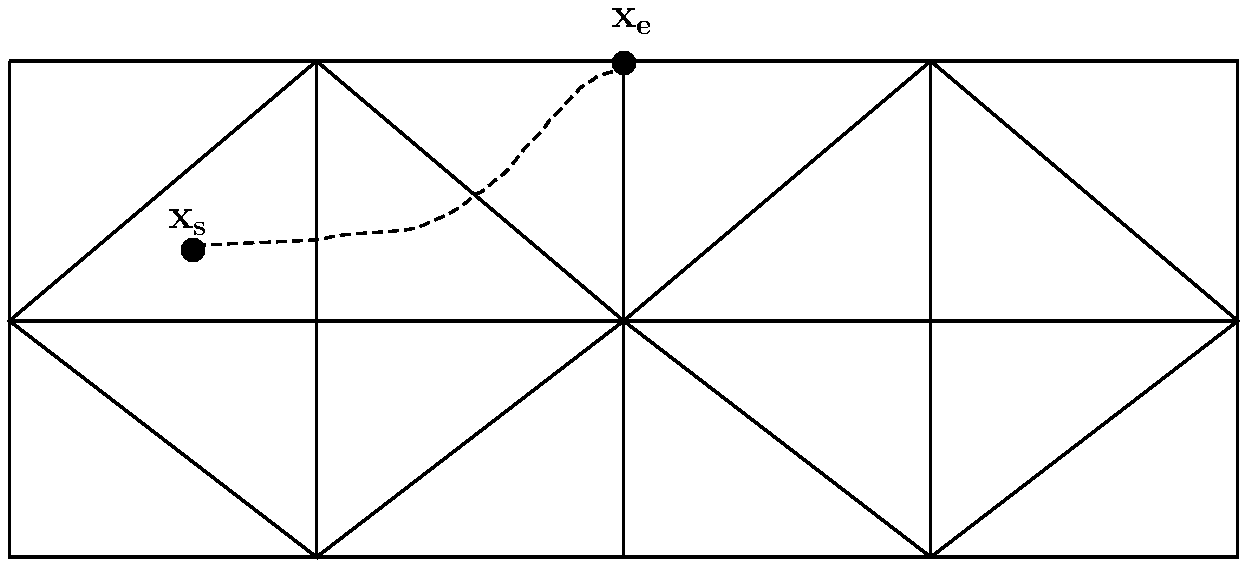
\includegraphics[width=0.7\linewidth]{../Figures/semi-lagrangian.pdf}
\end{figure}
\begin{align*}
\textbf{x}_s &= \textbf{x}_e - \Delta t \textbf{u}(\textbf{x}_e, t)
\end{align*}
\end{frame}
    
    
\begin{frame}{Дифузия -- слаба формулировка}
	\begin{align*}
		&\frac{\vecf{u}^B - \vecf{u}^A}{\Delta t} =\nu \Delta \vecf{u}^B, &&\left(\vecf{x}, t\right) \in \Omega \times J\\
		&\vecf{n} \cdot \grad{\vecf{u}^B} = 0, && \left(\vecf{x}, t\right) \in \Gamma_2 \times J \\
		&\vecf{u}^B = 0, &&\left(\vecf{x}, t\right) \in \left(\Gamma_1 \cup \Gamma_3 \cup \Gamma_5\right) \times J \\
		&\vecf{u}^B = \vecf{u}_{\Gamma_4}, && \left(\vecf{x}, t\right) \in \Gamma_4 \times J \\
	\end{align*}

	Тестово пространство: $\vecf{v} \in V : \left\{\vecf{v} \in H^1 : \vecf{v}(\vecf{x}, t)|_{\Gamma_D} = 0 \right\}$
	
	Търсим $\vecf{u} \in U : \left\{\vecf{v} \in H^1 : \vecf{v}(\vecf{x}, t)|_{\Gamma_1 \cup \Gamma_3 \cup \Gamma_5} = 0\right\}$, такова че:
	$$
	\dotprod{\frac{\vecf{u}^{B} - \vecf{u}^{A}}{\Delta t}}{\vecf{v}} = \dotprod{\nu\lapl{\vecf{u}^B}}{\vecf{v}}, \forall\vecf{v} \in V
	$$
\end{frame}

\begin{frame}{Дифузия -- МКЕ}
	\begin{align*}
		\dotprod{\vecf{u}^B}{\vecf{v}} = \dotprod{\vecf{u}^A}{\vecf{v}} - \Delta t \nu\left(\grad{\vecf{u}^B} : \grad{\vecf{v}}\right), \forall\vecf{v} \in V \\
		\dotprod{\vecf{u}^B}{\vecf{v}} + \Delta t \nu\left(\grad{\vecf{u}^B} : \grad{\vecf{v}}\right) = \dotprod{\vecf{u}^A}{\vecf{v}}, \forall\vecf{v} \in V
	\end{align*}
	Търсим приближеното решение: $\vecf{u}_h = \sum\limits_{i=1}^{2N_v}{\textbf{\textPhi}_iq_i} \in U_h$
	$$
	\left(\begin{bmatrix}
		\mathbf{M} & 0 \\
		0 & \mathbf{M}
	\end{bmatrix} + \nu\Delta t\begin{bmatrix}
		\mathbf{K} & 0 \\
		0 & \mathbf{K}
	\end{bmatrix}\right)\begin{bmatrix}
		\vecf{Q}^{B}_1 \\
		\vecf{Q}^{B}_2
	\end{bmatrix} = \begin{bmatrix}
		\mathbf{M} & 0 \\
		0 & \mathbf{M}
	\end{bmatrix}\begin{bmatrix}
		\vecf{Q}^{A}_1 \\
		\vecf{Q}^{A}_2
	\end{bmatrix}
	$$

\end{frame}

\begin{frame}{Налягане -- слаба формулировка}
	Основно уравнение:
	\begin{align*}
		&\frac{\vecf{u}^{i+1} - \vecf{u}^B}{\Delta t} = -\nabla p^i, &&\left(\vecf{x}, t\right) \in \Omega \times J\\
		&\vecf{n} \cdot \grad{p^i} = 0, && \left(\vecf{x}, t\right) \in (\Gamma_1 \cup \Gamma_3 \cup \Gamma_4 \cup \Gamma_5) \times J \\
		&p^i = 0, && \left(\vecf{x}, t\right) \in \Gamma_2 \times J
	\end{align*}
	Използваме $\nabla \cdot \textbf{u}^{i+1} = 0$ и вземаме дивергенцията на двете страни:
	$$
		\divg{\vecf{u}^B} = \lapl{p^i} \Delta t
	$$
	Умножаваме двете страни с функция от тестовото пространство: $q \in Q : \left\{q \in H^1 : q|_{\Gamma_2} = 0\right\}$. Решението търсим в пространството $Q$.
	$$
		\dotprod{\divg{\vecf{u}^B}}{q} = - \Delta t \dotprod{\grad{p^i}}{\grad{q}}, \forall q \in Q
	$$
\end{frame}

\begin{frame}{Налягане -- МКЕ}
	Търсим приближеното решение за налягането $p_h = \sum\limits_{i=1}^{N_p}{\chi_ip_i} \in Q_h$
	$$
	\begin{bmatrix}
		\mathbf{M} & 0 \\
		0 & \mathbf{M}
	\end{bmatrix} \begin{bmatrix}
		\vecf{Q}^{i+1}_1 \\
		\vecf{Q}^{i+1}_2
	\end{bmatrix} =	\begin{bmatrix}
		\mathbf{M} & 0 \\
		0 & \mathbf{M}
	\end{bmatrix} \begin{bmatrix}
		\vecf{Q}^{B}_1 \\
		\vecf{Q}^{B}_2
	\end{bmatrix} - \Delta t \begin{bmatrix}
		\vecf{B}_{p,1} \\
		\vecf{B}_{p,2}
	\end{bmatrix} \vecf{P}^i
	$$
\end{frame}

\begin{frame}{Намиране на $\textbf{u}^{i+1}$ -- Слаба формулировка}
Основно уравнение:
\begin{align*}
		&\frac{\vecf{u}^{i+1} - \vecf{u}^B}{\Delta t} = -\nabla p^i, &&\left(\vecf{x}, t\right) \in \Omega \times J\\
		&\vecf{n} \cdot \grad{\vecf{u}^i} = 0, && \left(\vecf{x}, t\right) \in \Gamma_2 \times J \\
		&\vecf{u}^i = 0, &&\left(\vecf{x}, t\right) \in \left(\Gamma_1 \cup \Gamma_3 \cup \Gamma_5\right) \times J \\
		&\vecf{u}^i = \vecf{u}_{\Gamma_4}, && \left(\vecf{x}, t\right) \in \Gamma_4 \times J \\
\end{align*}

	Тестово пространство: $\vecf{v} \in V : \left\{\vecf{v} \in H^1 : \vecf{v}(\vecf{x}, t)|_{\Gamma_D} = 0 \right\}$.
	
	Търсим $\vecf{u} \in U : \left\{\vecf{v} \in H^1 : \vecf{v}(\vecf{x}, t)|_{\Gamma_1 \cup \Gamma_3 \cup \Gamma_5} = 0\right\}$, такова че:
	$$
	\dotprod{\vecf{u}^{i+1}}{\vecf{v}} = \dotprod{\vecf{u}^B}{\vecf{v}} - \Delta t\dotprod{\vecf{v}} {\grad{p^i}}
	$$

\end{frame}


\begin{frame}{Намиране на $\textbf{u}^{i+1}$ -- МКЕ}
	Търсим приближеното решение: $\vecf{u}_h = \sum\limits_{i=1}^{2N_v}{\vecf{\textPhi}_iq_i} \in U_h$
	$$
	\begin{bmatrix}
		\mathbf{M} & 0 \\
		0 & \mathbf{M}
	\end{bmatrix} \begin{bmatrix}
		\vecf{Q}^{i+1}_1 \\
		\vecf{Q}^{i+1}_2
	\end{bmatrix} =	\begin{bmatrix}
		\mathbf{M} & 0 \\
		0 & \mathbf{M}
	\end{bmatrix} \begin{bmatrix}
		\vecf{Q}^{B}_1 \\
		\vecf{Q}^{B}_2
	\end{bmatrix} - \Delta t \begin{bmatrix}
		\vecf{B}_{p,1} \\
		\vecf{B}_{p,2}
	\end{bmatrix} \vecf{P}^i
	$$
\end{frame}
\iffalse
    \begin{frame}{Метод на крайните елементи -- обощение}
        	Търсим приближени решения за скоростта и налягането:
    		\begin{itemize}
    			\item $\vecf{u}_h = \sum\limits_{i=1}^{2N_v}{\vecf{\textPhi}_iq_i} \in U_h$
    			\item $p_h = \sum\limits_{i=1}^{N_p}{\chi_ip_i} \in L_h$
		\end{itemize}
        	\begin{align*}
	&\vecf{Q}^A = advect(KDTree, \vecf{Q}^i, \Delta t)\\
		&\left(\begin{bmatrix}
		\mathbf{M} & 0 \\
		0 & \mathbf{M}
	\end{bmatrix} + \nu\Delta t\begin{bmatrix}
		\mathbf{K} & 0 \\
		0 & \mathbf{K}
	\end{bmatrix}\right)\begin{bmatrix}
		\vecf{Q}^{B}_1 \\
		\vecf{Q}^{B}_2
	\end{bmatrix} = \begin{bmatrix}
		\mathbf{M} & 0 \\
		0 & \mathbf{M}
	\end{bmatrix}\begin{bmatrix}
		\vecf{Q}^{A}_1 \\
		\vecf{Q}^{A}_2
	\end{bmatrix}\\
	&\mathbf{K_p}\vecf{P}^i = -\frac{1}{\Delta t} \begin{bmatrix}
		\mathbf{B_1} & \mathbf{B_2}
	\end{bmatrix} \begin{bmatrix}
		\vecf{Q}^{B}_1 \\
		\vecf{Q}^{B}_2
	\end{bmatrix}\\
	&\begin{bmatrix}
		\mathbf{M} & 0 \\
		0 & \mathbf{M}
	\end{bmatrix} \begin{bmatrix}
		\vecf{Q}^{i+1}_1 \\
		\vecf{Q}^{i+1}_2
	\end{bmatrix} =	\begin{bmatrix}
		\mathbf{M} & 0 \\
		0 & \mathbf{M}
	\end{bmatrix} \begin{bmatrix}
		\vecf{Q}^{B}_1 \\
		\vecf{Q}^{B}_2
	\end{bmatrix} - \Delta t \begin{bmatrix}
		\vecf{B}_{p,1} \\
		\vecf{B}_{p,2}
	\end{bmatrix} \vecf{P}^i
\end{align*}
    \end{frame}
    
   
    \subsection{Избор на крайни елементи}
    \begin{frame}{Избор на крайни елементи}
\begin{columns} 
% Column 1
    \begin{column}{.5\textwidth}
        \begin{figure}[H]
  \centering
  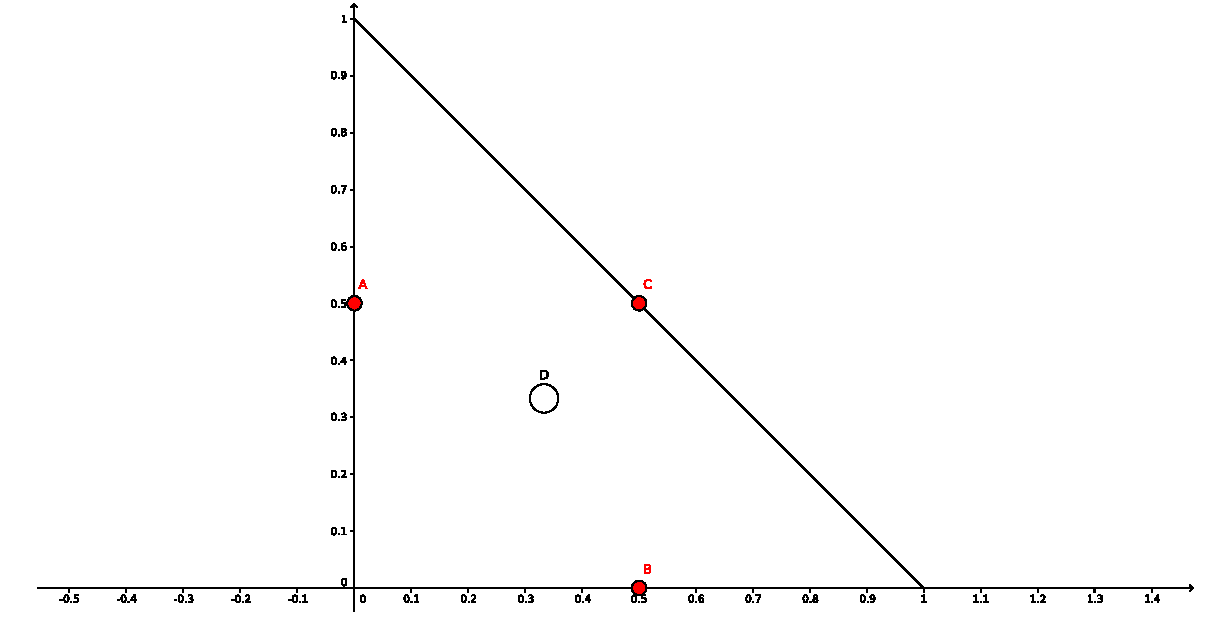
\includegraphics[width=\textwidth]{../Figures/01_introduction/cr_element.pdf}
  \caption{$P_{-1}P_0$ неконформен елемент на Crouzeix-Raviart}
\end{figure}
    \end{column}
% Column 2    
    \begin{column}{.5\textwidth}
\begin{figure}[H]
  \centering
  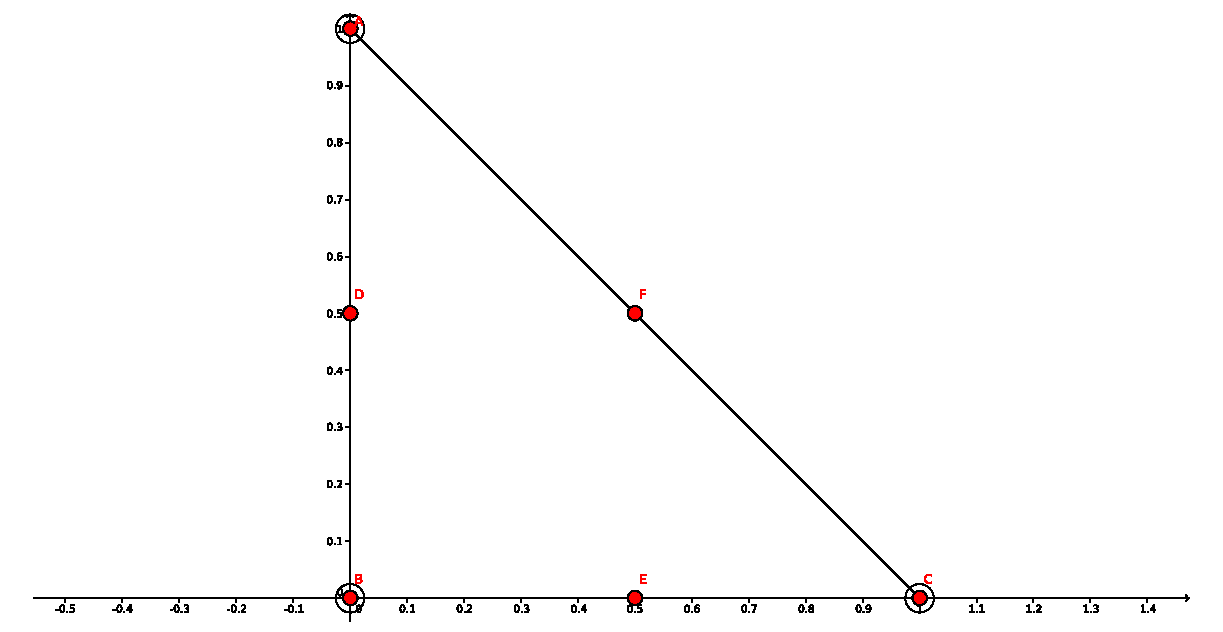
\includegraphics[width=\textwidth]{../Figures/01_introduction/tylor_hood_element.pdf}
  \caption{$P_2P_1$ елемент на Taylor-Hood}
\end{figure}
    \end{column}%

\end{columns}
    \end{frame}
    
\subsection{Числен експеримент}
	\begin{frame}{Числен експеримент}
	Решение за ламинарен поток след 100 стъпки с $\Delta t = 0.01, \nu=0.001$
	\begin{figure}[H]
\centering
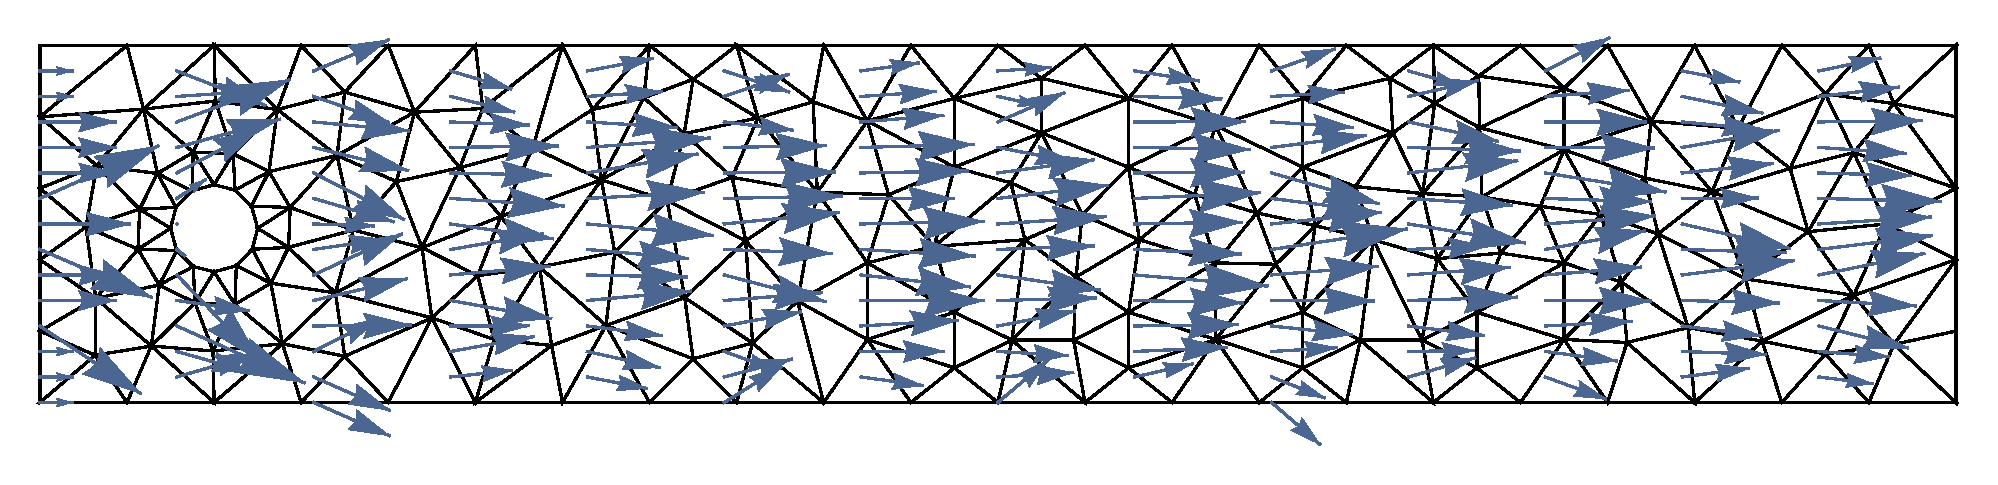
\includegraphics[width=0.8\textwidth]{../Figures/01_introduction/P1P0_100.pdf}
\end{figure}

\begin{figure}[H]
\centering
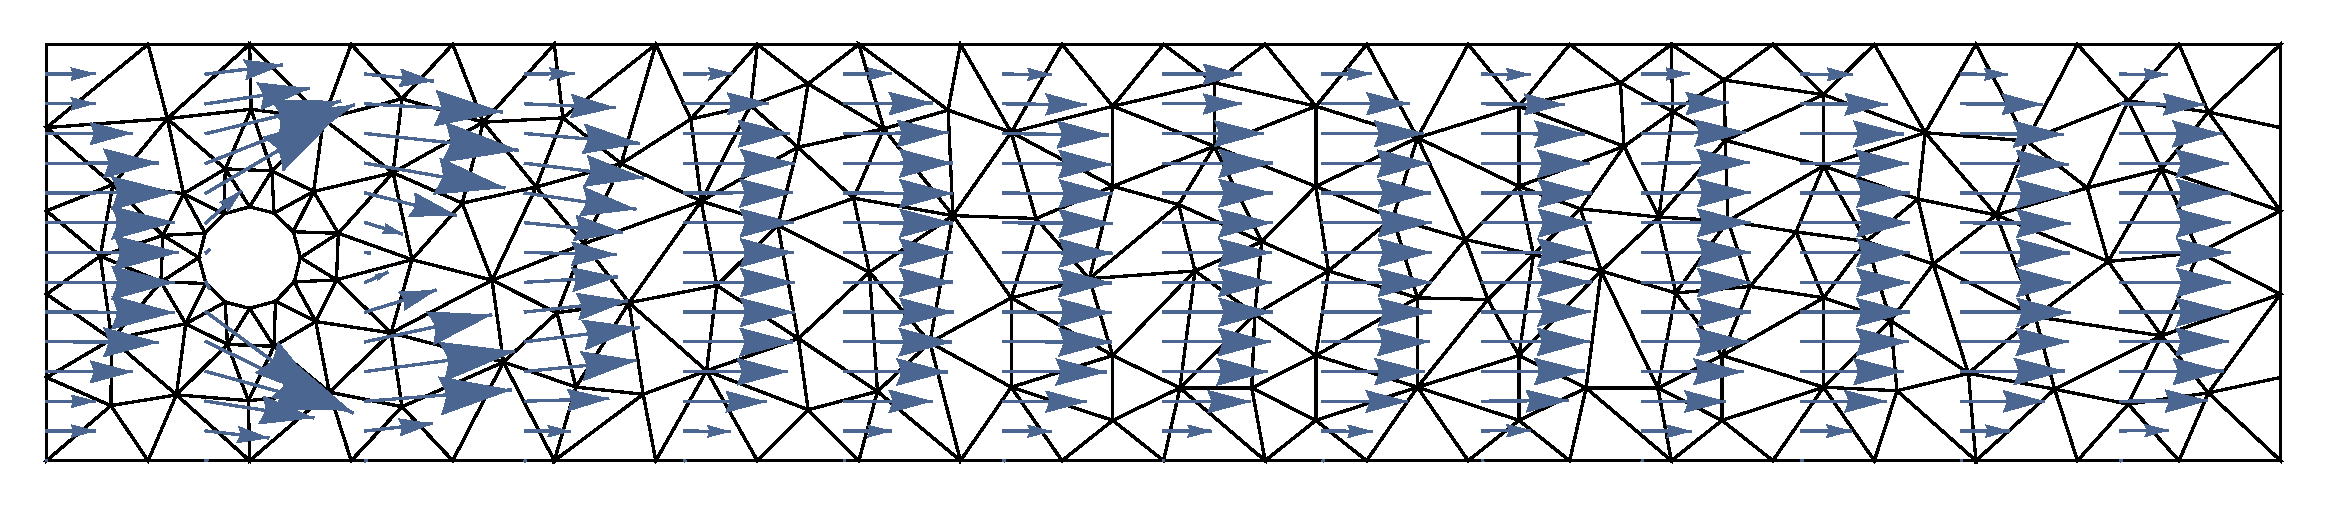
\includegraphics[width=0.8\textwidth]{../Figures/01_introduction/P2P1_100.pdf}
\end{figure}

\begin{figure}[H]
\centering
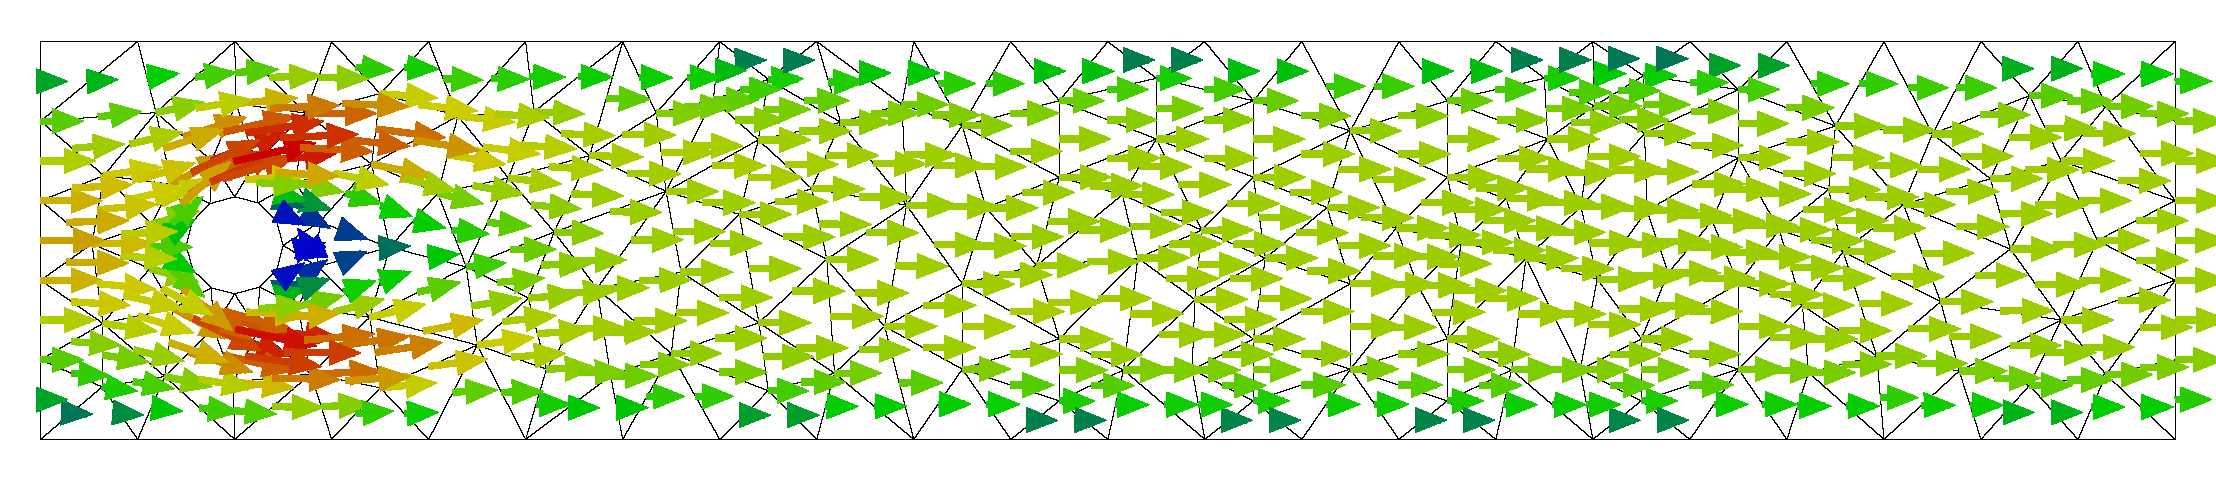
\includegraphics[width=0.8\textwidth]{../Figures/01_introduction/P2P1_adv_diff_100.pdf}
\end{figure}
	\end{frame}
	
\fi

\section{CPU Имплементация}
\subsection{Време за изпълнение -- CPU}
\begin{frame}{Време за изпълнение за ламинарен поток ($Re = 20$) -- CPU}
\begin{table}[H]
\centering
\begin{adjustbox}{max width=\textwidth}
\begin{tabular}{|c|c|c|c|c|c|c|c|}
\hline
\multirow{3}{*}{} & \multicolumn{7}{c|}{Компютър 2 -- 1 нишка}                                                                                                                                       
\\ \cline{2-8}
& Адвекция & Дифузия & \begin{tabular}[c]{@{}c@{}}Намиране на \\ налягането\end{tabular} & \begin{tabular}[c]{@{}c@{}}Намиране на \\ $\vecf{u}^{i+1}$\end{tabular} & \begin{tabular}[c]{@{}c@{}}СГ \\ (Общо)\end{tabular} & Асемблиране & \begin{tabular}[c]{@{}c@{}}Общо\\Време\end{tabular} \\ \hline
\begin{tabular}[c]{{@{{}}c@{{}}}}Средно\\време\end{tabular}  & 60.32s & 101.12s & 398.50s & 30.31s & 529.93s & 11.82s & 605.48s\\ \hline 
% \begin{tabular}[c]{@{}c@{}}Стандартно\\отклонение\end{tabular} & 0.15s&0.57s&1.85s&0.05s&2.14s&0.04s&2.27s\\ \hline 
% Медиана & 60.31s&100.96s&398.29s&30.33s&529.86s&11.84s&605.45s\\ \hline 
% Мин. & 60.03s&100.56s&395.98s&30.19s&526.75s&11.76s&602.09s\\ \hline 
% Макс & 60.54s&102.54s&402.81s&30.37s&534.01s&11.87s&609.62s\\ \hline
\end{tabular}\end{adjustbox}
\end{table}

\begin{table}[H]
\centering
\begin{adjustbox}{max width=\textwidth}
\begin{tabular}{|c|c|c|c|c|c|c|c|}
\hline
\multirow{3}{*}{} & \multicolumn{7}{c|}{Компютър 2 -- 8 нишки}                                                                                                                                       
\\ \cline{2-8}
& Адвекция & Дифузия & \begin{tabular}[c]{@{}c@{}}Намиране на \\ налягането\end{tabular} & \begin{tabular}[c]{@{}c@{}}Намиране на \\ $\vecf{u}^{i+1}$\end{tabular} & \begin{tabular}[c]{@{}c@{}}СГ \\ (Общо)\end{tabular} & Асемблиране & \begin{tabular}[c]{@{}c@{}}Общо\\Време\end{tabular} \\ \hline
\begin{tabular}[c]{{@{{}}c@{{}}}}Средно\\Време\end{tabular}&9.21s & 26.31s & 75.57s & 8.29s & 110.17s & 3.72s & 124.40s\\ \hline
% \begin{tabular}[c]{@{}c@{}}Стандартно \\ Отклонение\end{tabular} & 0.01s&0.21s&0.42s&0.03s&0.43s&0.02s&0.41s\\ \hline
% Медиана & 9.21s&26.26s&75.56s&8.27s&110.16s&3.72s&124.38s\\ \hline
% Мин. & 9.19s&26.04s&74.91s&8.24s&109.43s&3.70s&123.68s\\ \hline
% Макс. & 9.23s&26.70s&76.31s&8.33s&110.83s&3.78s&125.09s\\ \hline
\end{tabular}\end{adjustbox}
\end{table}
\end{frame}
\subsection{Асемблиране на глобалните матрици}





\iffalse
\begin{frame}{CSR формат за разредени матрици}

\begin{columns} 
% Column 1
    \begin{column}{.3\textwidth}
    \begin{figure}[H]
$$
\begin{bmatrix}
	1 & 0 & 0 & 2 & 0\\
	0 & 0 & 3 & 4 & 0\\
	0 & 0 & 5 & 0 & 6\\
	0 & 0 & 0 & 0 & 0\\
	7 & 0 & 8 & 9 & 0
\end{bmatrix}
$$
\caption{Примерна разредена матрица}
\end{figure}
    \end{column}
% Column 2    
    \begin{column}{.7\textwidth}
    \begin{figure}[H]
\centering
\begin{tabular}{l|ccccccccc}
\cline{2-10}
\textit{NZ}    & 1 & 2 & 3 & 4 & 5 & 6                      & 7 & 8 & \multicolumn{1}{c|}{9} \\ \cline{2-10}
\textit{Pos}   & 0 & 3 & 2 & 3 & 2 & 4                      & 0 & 2 & \multicolumn{1}{c|}{3} \\ \cline{2-10}
\textit{Start} & 0 & 2 & 4 & 6 & 6 & \multicolumn{1}{c|}{9} &   &   &                        \\ \cline{2-7}
\end{tabular}
\caption{Примерна разредена матрица в CSR формат}
\end{figure}
    \end{column}%
\end{columns}

\end{frame}
\fi






\begin{frame}{Асемблиране на глобалните матрици -- CPU}
	\begin{itemize}
		\item CSR формата налага зависимост между данните
		\item Матриците са константни
		\item Всяка матрица се пресмята на отделна нишка
	\end{itemize}
\end{frame}
\subsection{Адвекция}
\begin{frame}{Адвекция -- Паралелна имплементация}
	Задачата е тривиална.
	\begin{itemize}
		\item Разделяме възлите на $m$ групи
		\item Всяка нишка може независимо да намери скоростите за възлите от своята група
	\end{itemize}
\end{frame}
\begin{frame}{Адвекция -- паралелна имплементация, ламинарен поток}
        \begin{figure}[htbp]
            \centering
            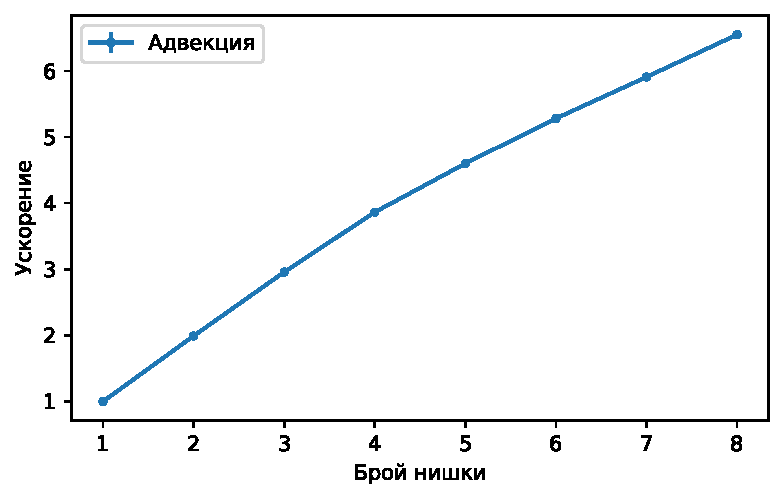
\includegraphics[width=\linewidth]{../Figures/BG/LaminarAdvectionSpeedUpC2.pdf} 
        \end{figure}
\end{frame}
%\begin{frame}{Адвекция -- паралелна имплементация, турбулентен поток}
%        \begin{figure}[htbp]
%            \centering
%            \subfigure{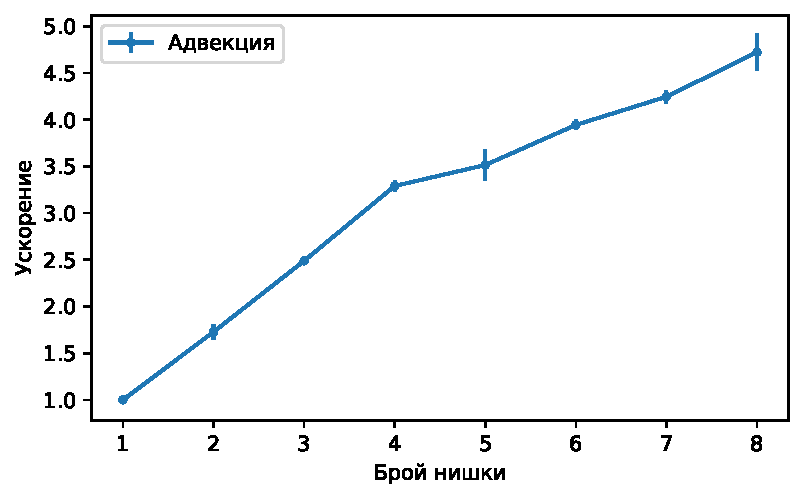
\includegraphics[width=0.49\linewidth]{../Figures/BG/TurbulentAdvectionSpeedUpC1.pdf}}
%            \subfigure{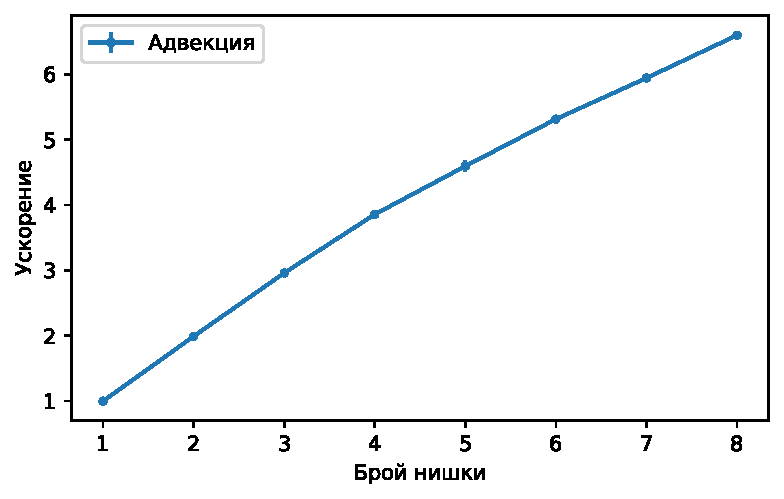
\includegraphics[width=0.49\linewidth]{../Figures/BG/TurbulentAdvectionSpeedUpC2.pdf}}      
%        \end{figure}
%\end{frame}
\subsection{Метод на спрегнатия градиент}
\begin{frame}{Метод на спрегнатия градиент -- CPU}
	\begin{itemize}
		\item Нужни са сихронизационни примитиви
		\item Всяка част от една стъпка е тривиална за паралелна имплементация
	\end{itemize}
\end{frame}
\begin{frame}{Метод на спрегнатия градиент -- алгоритъм}
\begin{algorithm}[H]
\centering
\floatname{algorithm}{Алгоритъм}
\caption{Метод на спрегнатия градиент за решаване на $Ax=b$ с начално приближение $x_0$}
    \begin{algorithmic}[1]
		\Procedure{CG}{$A, b, x_0$}
			\State $r_0 \gets b - Ax_0$
			\State $p_0 \gets r_0$
			\For{$j \gets 0, 1, \dots$ until convergence}
				\State $ap \gets Ap_j$
				\State $\alpha_j \gets \frac{(r_j, r_j)}{(ap, p_j)}$
				\State $x_{j+1} \gets x_j + \alpha_j p_j$
				\State $r_{j+1} \gets r_j - \alpha_j ap$
				\State $\beta_j \gets \frac{(r_{j+1}, r_{j+1})}{(r_j, r_j)}$
				\State $p_{j+1} \gets r_{j+1} + \beta_j p_j$
			\EndFor
			\State \Return $x_{j+1}$
		\EndProcedure
    \end{algorithmic}
\end{algorithm}
\end{frame}
\begin{frame}{Метод на спрегнатия градиент -- паралелна имплементация, ламинарен поток ($Re = 20$)}
\begin{figure}[H]
            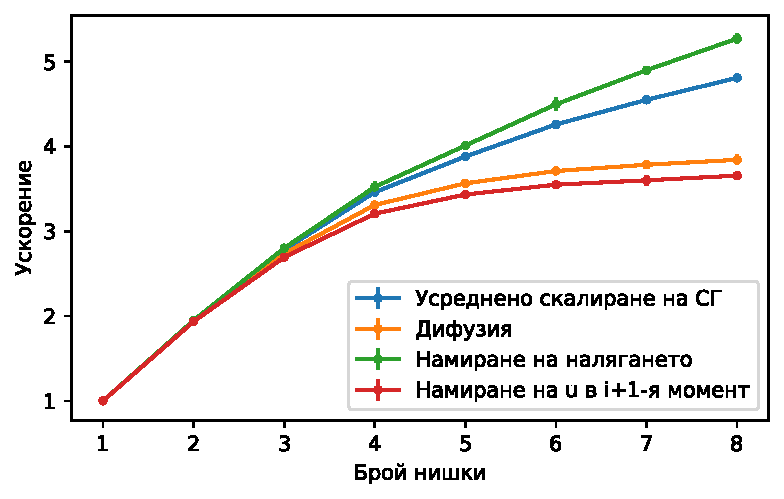
\includegraphics[width=\linewidth]{../Figures/BG/LaminarCGSpeedUpC2.pdf}   
\end{figure}
\end{frame}
%\begin{frame}{Метод на спрегнатия градиент -- паралелна имплементация, турбулентен поток}
%\begin{figure}[H]
%            \subfigure{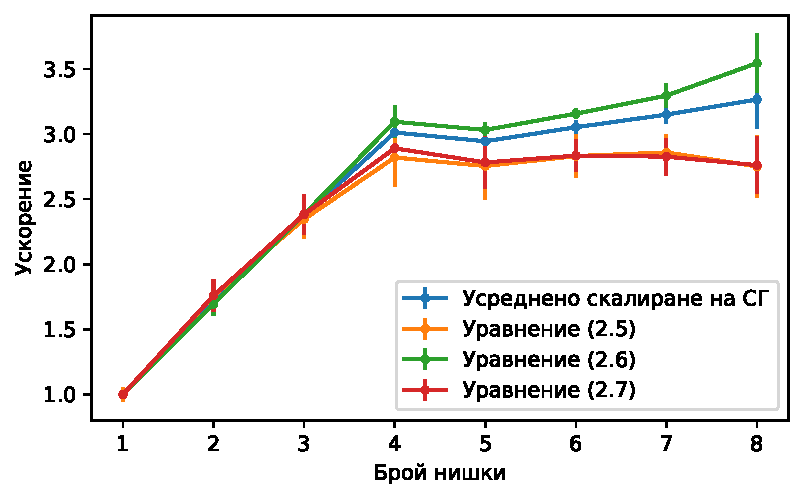
\includegraphics[width=0.49\linewidth]{../Figures/BG/TurbulentCGSpeedUpC1.pdf}}
%            \subfigure{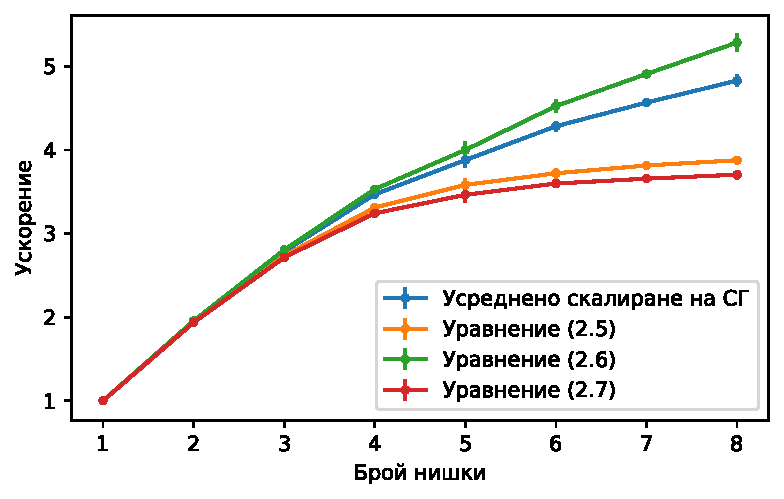
\includegraphics[width=0.49\linewidth]{../Figures/BG/TurbulentCGSpeedUpC2.pdf}}     
%\end{figure}
%\end{frame}
\iffalse
\begin{frame}{Метод на спрегнатия градиент -- преобуславяне}
	\begin{itemize}
		\item Намаляваме броя итерации
		\item Търсим $P^{-1} \approx A^{-1}$
		\item Непълна факторизация на Холецки. Пресмятане, проблеми
		\item Произведението на две разредени матрици не е разредена матрица
	\end{itemize}
\end{frame}
\begin{frame}{Метод на спрегнатия градиент -- преобуславяне, алгоритъм}
\begin{algorithm}[H]
\centering
\floatname{algorithm}{Алгоритъм}
\caption{Преобусловен метод на спрегнатия градиент за решаване на $Ax=b$ с начално приближение $x_0$}\label{alg:pcg}
\begin{algorithmic}[1]
		\Procedure{PCG}{$A, M^{-1} b, x_0$}
			\State $r_0 \gets b - Ax_0$
			\State $z_0 \gets M^{-1}r_0$\label{alg-line:apply-preconditioner}
			\State $p_0 \gets z_0$
			\For{$j \gets 0, 1, \dots$ until convergence}
				\State $\alpha_j \gets \frac{(r_j, z_j)}{(Ap_j, p_j)}$
				\State $x_{j+1} \gets x_j + \alpha_j p_j$
				\State $r_{j+1} \gets r_j - \alpha_j Ap_j$
				\State $z_{j+1} \gets M^{-1}r_{j+1}$
				\State $\beta_j \gets \frac{(r_{j+1}, z_{j+1})}{(r_j, z_j)}$
				\State $p_{j+1} \gets z_{j+1} + \beta_j p_j$
			\EndFor
			\State \Return $x_{j+1}$
		\EndProcedure
\end{algorithmic}
\end{algorithm}
\end{frame}

\begin{frame}{Метод на спрегнатия градиент -- преобуславяне, брой итерации}
\begin{table}[H]
\centering
\begin{adjustbox}{max width=\textwidth}
\begin{tabular}{|c|c|c|c|}
\hline Задача
& \begin{tabular}[c]{@{}c@{}}Брой итерации\\ Дифузия\end{tabular} & \begin{tabular}[c]{@{}c@{}}Брой итерации\\ намиране на налягането\end{tabular} & \begin{tabular}[c]{@{}c@{}}Брой итерации\\ прилагане на налягането\end{tabular} \\ \hline
Ламинарен поток ($Re = 20$)         & 10370& 195422 &    2763 \\ \hline
%Турбулентен поток       & 14820& 264394 &   3504 \\ \hline
Ламинарен поток ($Re = 20$) с IC0   &  1855&  72353 &    495\\ \hline
%Турбулентен поток (IC0) &  2693&  85047 &    693\\ \hline
\end{tabular}\end{adjustbox}\caption{Общ брой итерации за всяка една система.}
\end{table}
\end{frame}

\begin{frame}{Метод на спрегнатия градиент -- преобуславяне, време за пресмятане на IC0}
\begin{table}[H]
\centering
\begin{adjustbox}{max width=\textwidth}
\begin{tabular}{|c|c|c|c|c|c|}
\hline
                                                                                   & \begin{tabular}[c]{@{}c@{}}Средно\\ време\end{tabular} & Медиана & SD   & \begin{tabular}[c]{@{}c@{}}Мин.\\ време\end{tabular} & \begin{tabular}[c]{@{}c@{}}Макс.\\ време\end{tabular} \\ \hline
\begin{tabular}[c]{@{}c@{}}Пресмятане на IC0 за\\ Матрица на коравината на налягането\end{tabular} & 15.66                                               & 15.67  & 0.02 & 15.64                                              & 15.68                                              \\ \hline
\begin{tabular}[c]{@{}c@{}}Пресмятане IC0 за\\ Матрица на маста за скоростта\end{tabular}      & 390.33                                              & 389.98 & 1.32 & 389.22                                             & 391.79                                             \\ \hline
\begin{tabular}[c]{@{}c@{}}Пресмятане IC0 за\\ Дифузионна матрица\end{tabular}          & 380.68                                              & 379.17 & 4.98 & 376.62                                             & 386.23                                             \\ \hline
\end{tabular}\end{adjustbox}
\end{table}

Можем да пресметнем само за матрицата на коравина за налягането.

\end{frame}

\begin{frame}{Метод на спрегнатия градиент -- преобуславяне, време за решаване на системите, на 1 нишка }
\begin{table}[H]
\centering
\footnotesize
\begin{adjustbox}{max width=\textwidth}
\begin{tabular}{|c|c|c|c|c|c|}
\hline
     & \begin{tabular}[c]{@{}c@{}}Средно\\ Време\end{tabular} & Медиана & \begin{tabular}[c]{@{}c@{}}Стандартно \\ Отклонение\end{tabular}   & \begin{tabular}[c]{@{}c@{}}Минимално\\ Време\end{tabular} & \begin{tabular}[c]{@{}c@{}}Максимално\\ Време\end{tabular} \\ \hline
Дифузия & 101.12s & 100.96s & 0.57s & 100.56s & 102.54s \\ \hline
\begin{tabular}[c]{@{}c@{}}Намиране на \\ налягането\end{tabular} & 398.50s & 398.29 & 1.85s & 395.98s & 402.81s  \\ \hline
\begin{tabular}[c]{@{}c@{}}Прилагане на \\ налягането\end{tabular} & 30.31s & 30.33s  & 0.05s & 30.19s & 30.37s  \\ \hline

Дифузия (IC0) & 54.76s & 54.76s  & 0.00 & 54.76s & 74.75s \\ \hline
\begin{tabular}[c]{@{}c@{}}Намиране на \\ налягането (IC0)\end{tabular} & 393.30s & 393.50s & 0.29s & 393.09s & 393.50s  \\ \hline
\begin{tabular}[c]{@{}c@{}}Прилагане на \\ налягането (IC0)\end{tabular} & 22.01s & 22.03s  & 0.03s & 21.99s & 22.03s  \\ \hline
\end{tabular}\end{adjustbox}\caption{Ламинарен поток, компютър 2, 1 нишка.}
\end{table}

\end{frame}

\fi

\section{GPU имплементация}
\subsection{Хардуерна архитектура на графичните процесори}
\begin{frame}{GPU архитектура -- Streaming Multiprocessor}
\begin{columns} 
% Column 1
    \begin{column}{.5\textwidth}
        \begin{figure}[H]
  \centering
  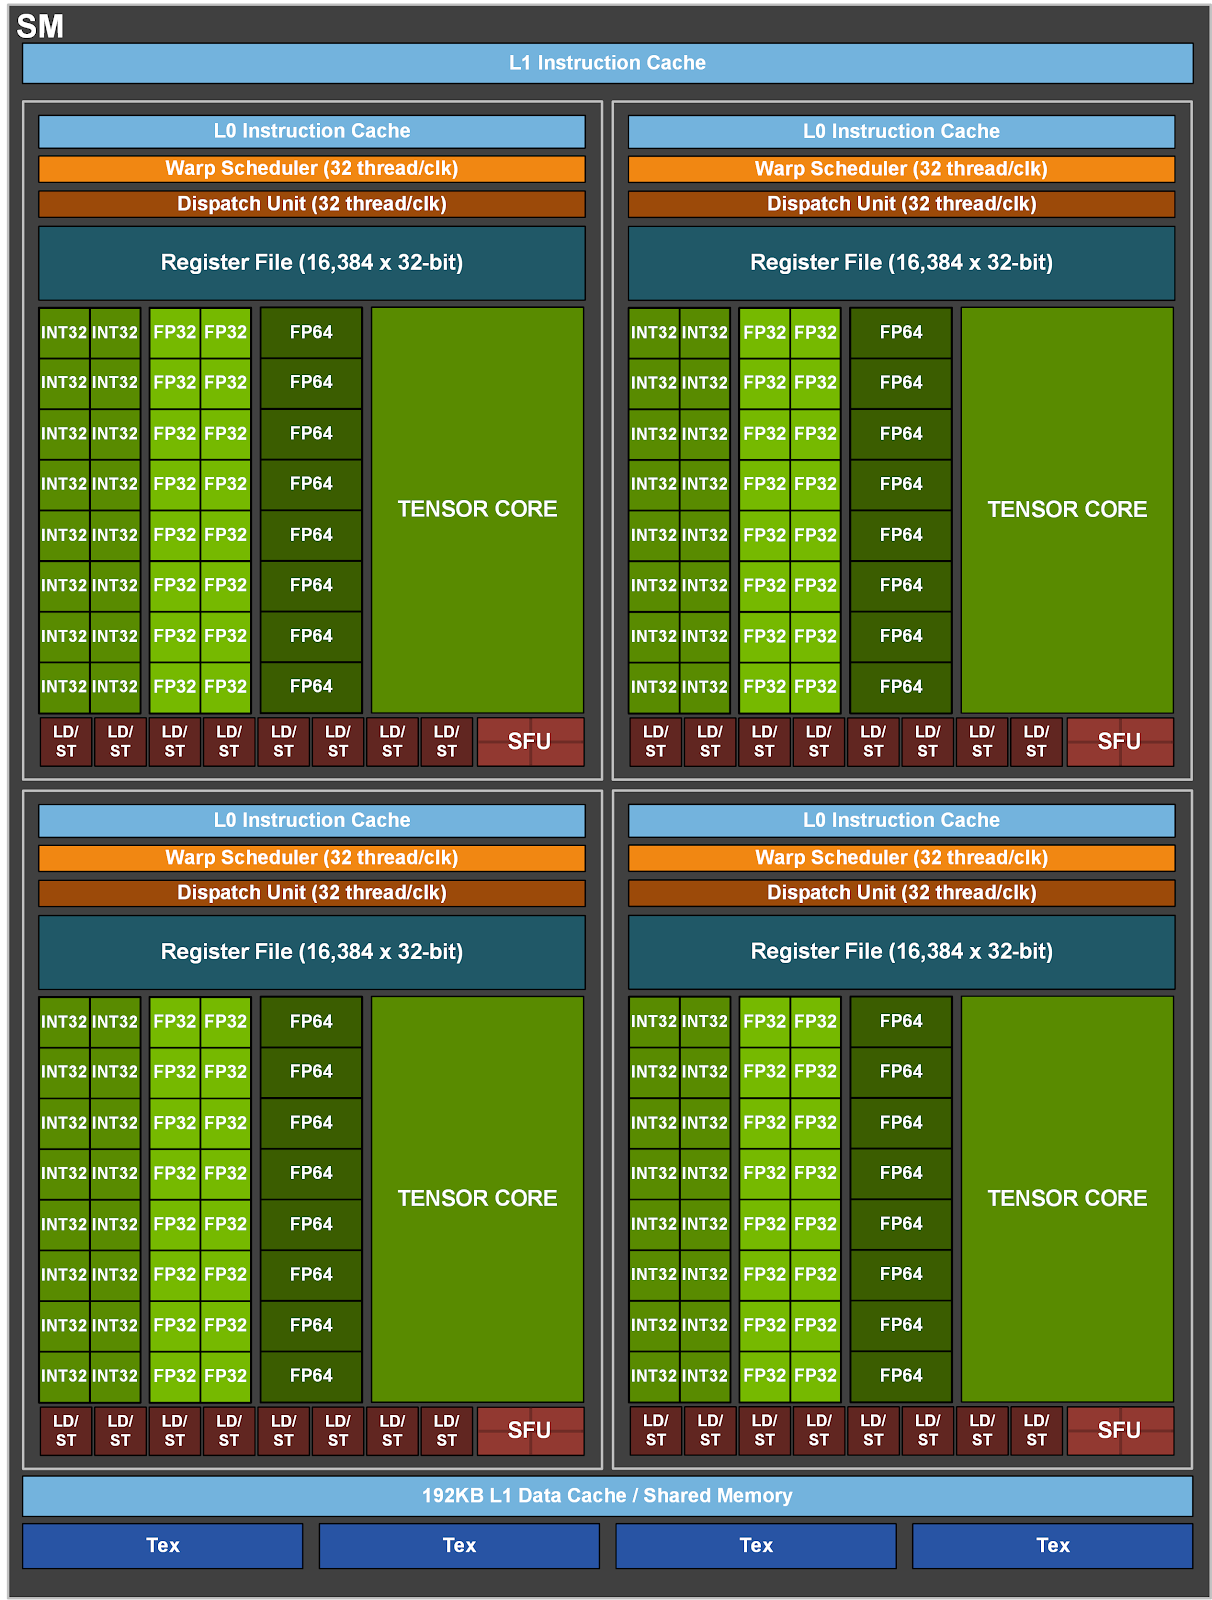
\includegraphics[width=0.95\textwidth]{../Figures/presentation/sm.png}
\end{figure}
    \end{column}
% Column 2    
    \begin{column}{.5\textwidth}
		\begin{itemize}
			\item 64 CUDA ядра
			\item Warp, active warp
			\item Условни оператори
		\end{itemize}
    \end{column}
\end{columns}
\end{frame}

\begin{frame}{GPU Цялостна архитектура}
   \begin{figure}[H]
  \centering
  \includegraphics[width=\textwidth]{../Figures/presentation/а100.png}
\end{figure}
\end{frame}
\begin{frame}{Програмен модел}
	\begin{itemize}
		\item Kernel
		\item Grid (2D/3D)
		\item Thread block (до 1024 нишки).
		\item Препоръчително е в един grid да има повече блокове отколкото SM
		\item Пример -- събиране на два вектора
	\end{itemize}
	\begin{table}[]
\begin{tabular}{llll}
$a_0$ & $a_1$ & $\dots$ & $a_n$ \\
\multicolumn{4}{c}{+} \\
$b_0$ & $b_1$ & $\dots$ & $b_n$
\end{tabular}
\end{table}
\end{frame}

\subsection{Адвекция}
\begin{frame}{GPU -- Адвекция}
	\begin{itemize}
		\item Пасва идеално на програмния модел
	\end{itemize}
\end{frame}
\subsection{Метод на спрегнатия градиент}
\begin{frame}{Метод на спрегнатия градиент -- Mega kernel подход}
	\begin{itemize}
		\item Сравнение с multi kernel подход
		\item Целият метод е един kernel
		\item Изисква сихнронизация
	\end{itemize}
\end{frame}
\begin{frame}{Време за изпълнение за ламинарен поток ($Re = 20$) -- GPU}
\begin{table}[H]
\centering
\begin{adjustbox}{max width=\textwidth}
\begin{tabular}{|c|c|c|c|c|c|c|c|}
\hline
\multirow{3}{*}{} & \multicolumn{7}{c|}{GPU Mega Kernel подход}                                                                                                                                       
\\ \cline{2-8}
& Адвекция & Дифузия & \begin{tabular}[c]{@{}c@{}}Намиране на \\ налягането\end{tabular} & \begin{tabular}[c]{@{}c@{}}Намиране на \\ $\vecf{u}^{i+1}$\end{tabular} & \begin{tabular}[c]{@{}c@{}}СГ \\ (Общо)\end{tabular} & Асемблиране & \begin{tabular}[c]{@{}c@{}}Общо\\Време\end{tabular} \\ \hline
\begin{tabular}[c]{{@{{}}c@{{}}}}Средно\\време\end{tabular}  & 0.54s & 2.98s & 8.19s & 1.26s & 12.44s & 4.02s & 18.24s\\ \hline
% \begin{tabular}[c]{@{}c@{}}Стандартно\\отклонение\end{tabular} & 0.01s&0.07s&0.09s&0.01s&0.06s&0.02s&0.06s\\ \hline
% Медиана & 0.54s&2.96s&8.20s&1.26s&12.43s&4.02s&18.22s\\ \hline
% Мин. & 0.53s&2.95s&7.95s&1.25s&12.36s&3.99s&18.13s\\ \hline
% Макс. & 0.55s&3.18s&8.29s&1.28s&12.54s&4.05s&18.32s\\ \hline
\end{tabular}\end{adjustbox}
\end{table}

\begin{figure}[H]
\centering
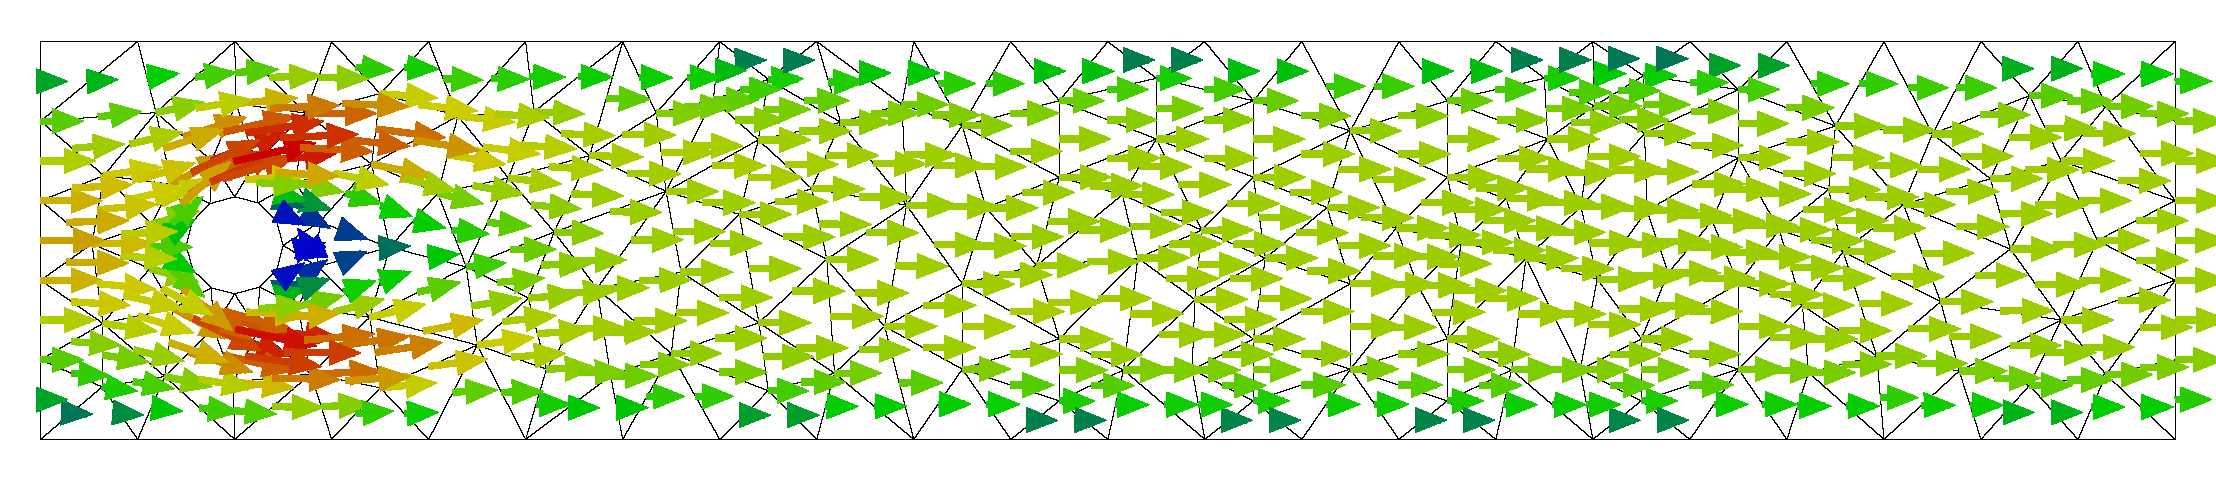
\includegraphics[width=\textwidth]{../Figures/01_introduction/P2P1_adv_diff_100.pdf}
\end{figure}

\end{frame}

\section{Заключение}
\begin{frame}{Заключение}
\begin{itemize}
	\item Представени са 3 метода за решаване на уравненията на Navier-Stokes
	\item Разделянето на диференциалния оператор по времето на 3 части пасва най-добре на зададените цели
	\item Полу-Лагранжевият метод за адвекция е подходящ за паралелна имплементация
	\item Ускорението от паралелна имплементация на метода на спрегнатия градиент се усеща най-добре за големи матрици и уравнения с много итерации
\end{itemize}
\end{frame}

\section{Насоки за развитие}
\begin{frame}{Насоки за развитие}
	\begin{itemize}
		\item Експерименти с други видове елементи
		\item Разделяне на оператора с по-голяма точност, напр. разделяне на Странг
		\item Апроксимация по времето с по-голяма точност, напр. методи на Рунге-Кута
		\item Използване на ``многоетапен'' полу-Лагранжев метод
		\item Паралелно асемблиране на глобалните матрици
		\item Паралелна имплементация на пресмятането и прилагането на IC0
		\item Разглеждане на други преобуславящи методи, напр. блочно пребуславяне на Якоби
	\end{itemize}
\end{frame}

\begin{frame}
	\centering
	\Large
	Благодаря за вниманието!
\end{frame}

\end{document}